
\subsection{Esempio Massa-Molla-Smorzatore con due masse}
Si vuole analizzare il modello ISU del seguente sistema composto da due masse
disposte nel seguente modo:
\begin{figure}[h]
 \centering
 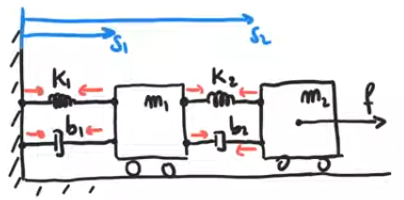
\includegraphics[width=\picwid]{massa_molla_smorzatore_esempio_2.png}
 \label{fig:massa_molla_smorzatore_esempio_2}
\end{figure}

Si individua il sistema di riferimento e si indica con $s_1$ la posizione della
prima massa ed $s_2$ la seconda.
Esiste un'unica direzione di movimento e sono presenti due masse, dunque si
scriveranno due equazioni.
$$\left\{\begin{aligned}
m_1\ddot{s}_1 &= k_2(s_2-s_1) + b_2(\dot{s}_2-\dot{s}_1) -k_1s_1 - b_1\dot{s}_1
\\
m_2\ddot{s}_2 &= f - k_2(s_2-s_1) - b_2(\dot{s}_2-\dot{s}_1)
\end{aligned}\right.$$

Si analizzano le variabili del sistema
$$\begin{matrix}
f & s_1& \dot{s}_1 & s_2 &\dot{s}_2 \\
(0) & (2) & & (2) \\
u & x_1 & x_2 & x_3 & x_4
\end{matrix}$$

L'ordine del sistema è dunque quattro $(n=4)$, dato che ogni variabile non di
ingresso viene differenziata due volte.

Si riscrivono le equazioni in forma ISU
$$\left\{\begin{aligned}
\dot{x}_1 &= \dot{s}_1 = x_2 \\
\dot{x}_2 &= \ddot{s}_1 = \frac{k_2}{m_1}(x_3-x_1) + \frac{b_2}{m_1} (x_4-x_2)
- \frac{k_1}{m_1}x_1 - \frac{b_1}{m_1}x_2\\
\dot{x}_3 &=\dot{s}_2 = x_4 \\
\dot{x}_4 &= \ddot{s}_2 = \frac{1}{m_2}u -\frac{k_2}{m_2}(x_3-x_1) -
\frac{b_2}{m_2}(x_4 - x_2)\\
\ &\text{Uscite assegnate}\\
y_1 &= s_1 = x_1 \\
y_2 &= s_2 = x_3
\end{aligned}\right.$$

\newpage
Il sistema è lineare tempo invariante strettamente causale, si può porre il
sistema in forma matriciale compatta
$$x =
\begin{pmatrix}
 x_1 \\ x_2 \\ x_3 \\ x_4
\end{pmatrix} \quad
y= \begin{pmatrix}
    y_1 \\ y_2
   \end{pmatrix}
$$
$$\text{ISU} = \left\{\begin{aligned}
\dot{x} &= \begin{pmatrix}
0 & 1 & 0 & 0 \\
\\
-\frac{k_1+k_2}{m_1} & -\frac{b_1+b_2}{m_1} &
\frac{k_2}{m_1} & \frac{b_2}{m_1}\\
\\
0 & 0 & 0 & 1\\ \\
\frac{k_2}{m_2} & \frac{b_2}{m_2} & -\frac{k_2}{m_2} & -\frac{b_2}{m_2}
          \end{pmatrix}x +
          \begin{pmatrix}
        0 \\ 0 \\ 0 \\ \frac{1}{m}
          \end{pmatrix}u\\
y &=      \begin{pmatrix}
           1 & 0 & 0 & 0 \\
           0 & 0 & 1 & 0
          \end{pmatrix}x
\end{aligned}\right.$$
27:58
